Finally, we examine performance of a Machine Learning (ML) algorithms. 
The goal of this experiment is to evaluate better memory management strategies in ML algorithms developed with Rust.
We employ K-Nearest-Neighbors (KNN) for ML algorithm to be studied in our experiments.
Our KNN algorithms perform document classification on Wikipedia page data set described in Section~\ref{sec:eval_setdetail}. 

The algorithms have 4 phase; load, preprocess, query, and combine phase. 
The algorithms spawn threads at the beginning ,and in the load phase partition of files are loaded in each threads. 
In preprocessing phase, the algorithm process document strings to generate Term-frequencies (Tfs) matrices and other data structures. 
In query phase, it calculates cosine similarities between all combination of train and test observations and select to top \(K\) nearest neighbors. 
In combine phase, the results from each batch and from each are combined. 
Based on our experiments result, the runtime in preprocess and query phase are significantly larger than other two phases.
Therefore, we focus discussion in these two phases considering them bottlenecks in our KNN algorithms.

KNN algorithms are implemented with different memory management strategies. 
We parametrize these memory management and some other values. These parameters are listed in Table~\ref{tab:parameter}. 

\begin{table}
    \renewcommand{\arraystretch}{1.2}
    \begin{tabular}{|l|l|l|l|l|}
    \hline
    Parameter Name  & \multicolumn{4}{l|}{Values and Description}                                                                                                                                                                                \\ \hline
    Method          & \multicolumn{4}{l|}{\begin{tabular}[c]{@{}l@{}}deep-copy:  use deep-copy to generate intermediate objects\\ arc: use atomic reference count to generate intermediate objects\end{tabular}}                                 \\ \hline
    Strategy        & \multicolumn{4}{l|}{\begin{tabular}[c]{@{}l@{}}1: keep intermediate objects in memory until owner is changed\\ 2: remove intermediate objects as soon as it is not needed\end{tabular}}                                    \\ \hline
    Number of batch & \multicolumn{4}{l|}{\begin{tabular}[c]{@{}l@{}}2: generate 2 batch from each partition\\ 3: generate 3 batch from each partition\end{tabular}}                                                                             \\ \hline
    k               & \multicolumn{4}{l|}{\begin{tabular}[c]{@{}l@{}}15K: dimension of feature matrices is 15 thousands \\ 20K: dimension of feature matrices is 20 thousands\\ 25K: dimension of feature matrices is 25 thousands\end{tabular}} \\ \hline
    \end{tabular}
    \caption{Parameter of KNN algorithms}
    \label{tab:parameter}
 \end{table}


Method parameter is specified to select memory management strategy used in preprocess phase. 
In preprocess phase, the algorithm generates many intermediate data structures using same String elements.
Deep-copy method deeply copies String to generate intermediate data structures. Arc method use Atomic Reference Count (Arc) to wrap String elements in the original data structure and 
clone Arc when the elements are used in other data structures. As Experiment 4 had shown in in Section~\ref{sec:eval_treeagg}, deep-copy of complex objects is more expensive than cloning Arc. 
String is a sort of objects allocated in heap and copied many times in preprocess phase. Therefore, it is worth to assess which method can be better memory management strategy in our experiments.

Strategy parameter controls memory management strategy used in both preprocess and query phase.
Strategy 1 keeps all intermediate data structures and numeric matrix objects from preprocess to query phase. 
Strategy 2 removes these data structures and objects as soon as they are not needed. 
These strategies differ from each other in terms of memory usage and frequency of memory deallocations.
These may cause significant runtime difference of the algorithms.

Number of batch controls number and size of batch for each partition. This parameter varies size of intermediate data structures and numeric matrices, and 
frequency of memory deallocations. Parameter k specifies dimension of feature matrices. This determines size of intermediate data structures and numeric matrices.

By controlling these parameter, we compare runtime and memory usage of KNN algorithms. 


\subsection{Result}
\label{sec:history}



\begin{figure}[htb]
    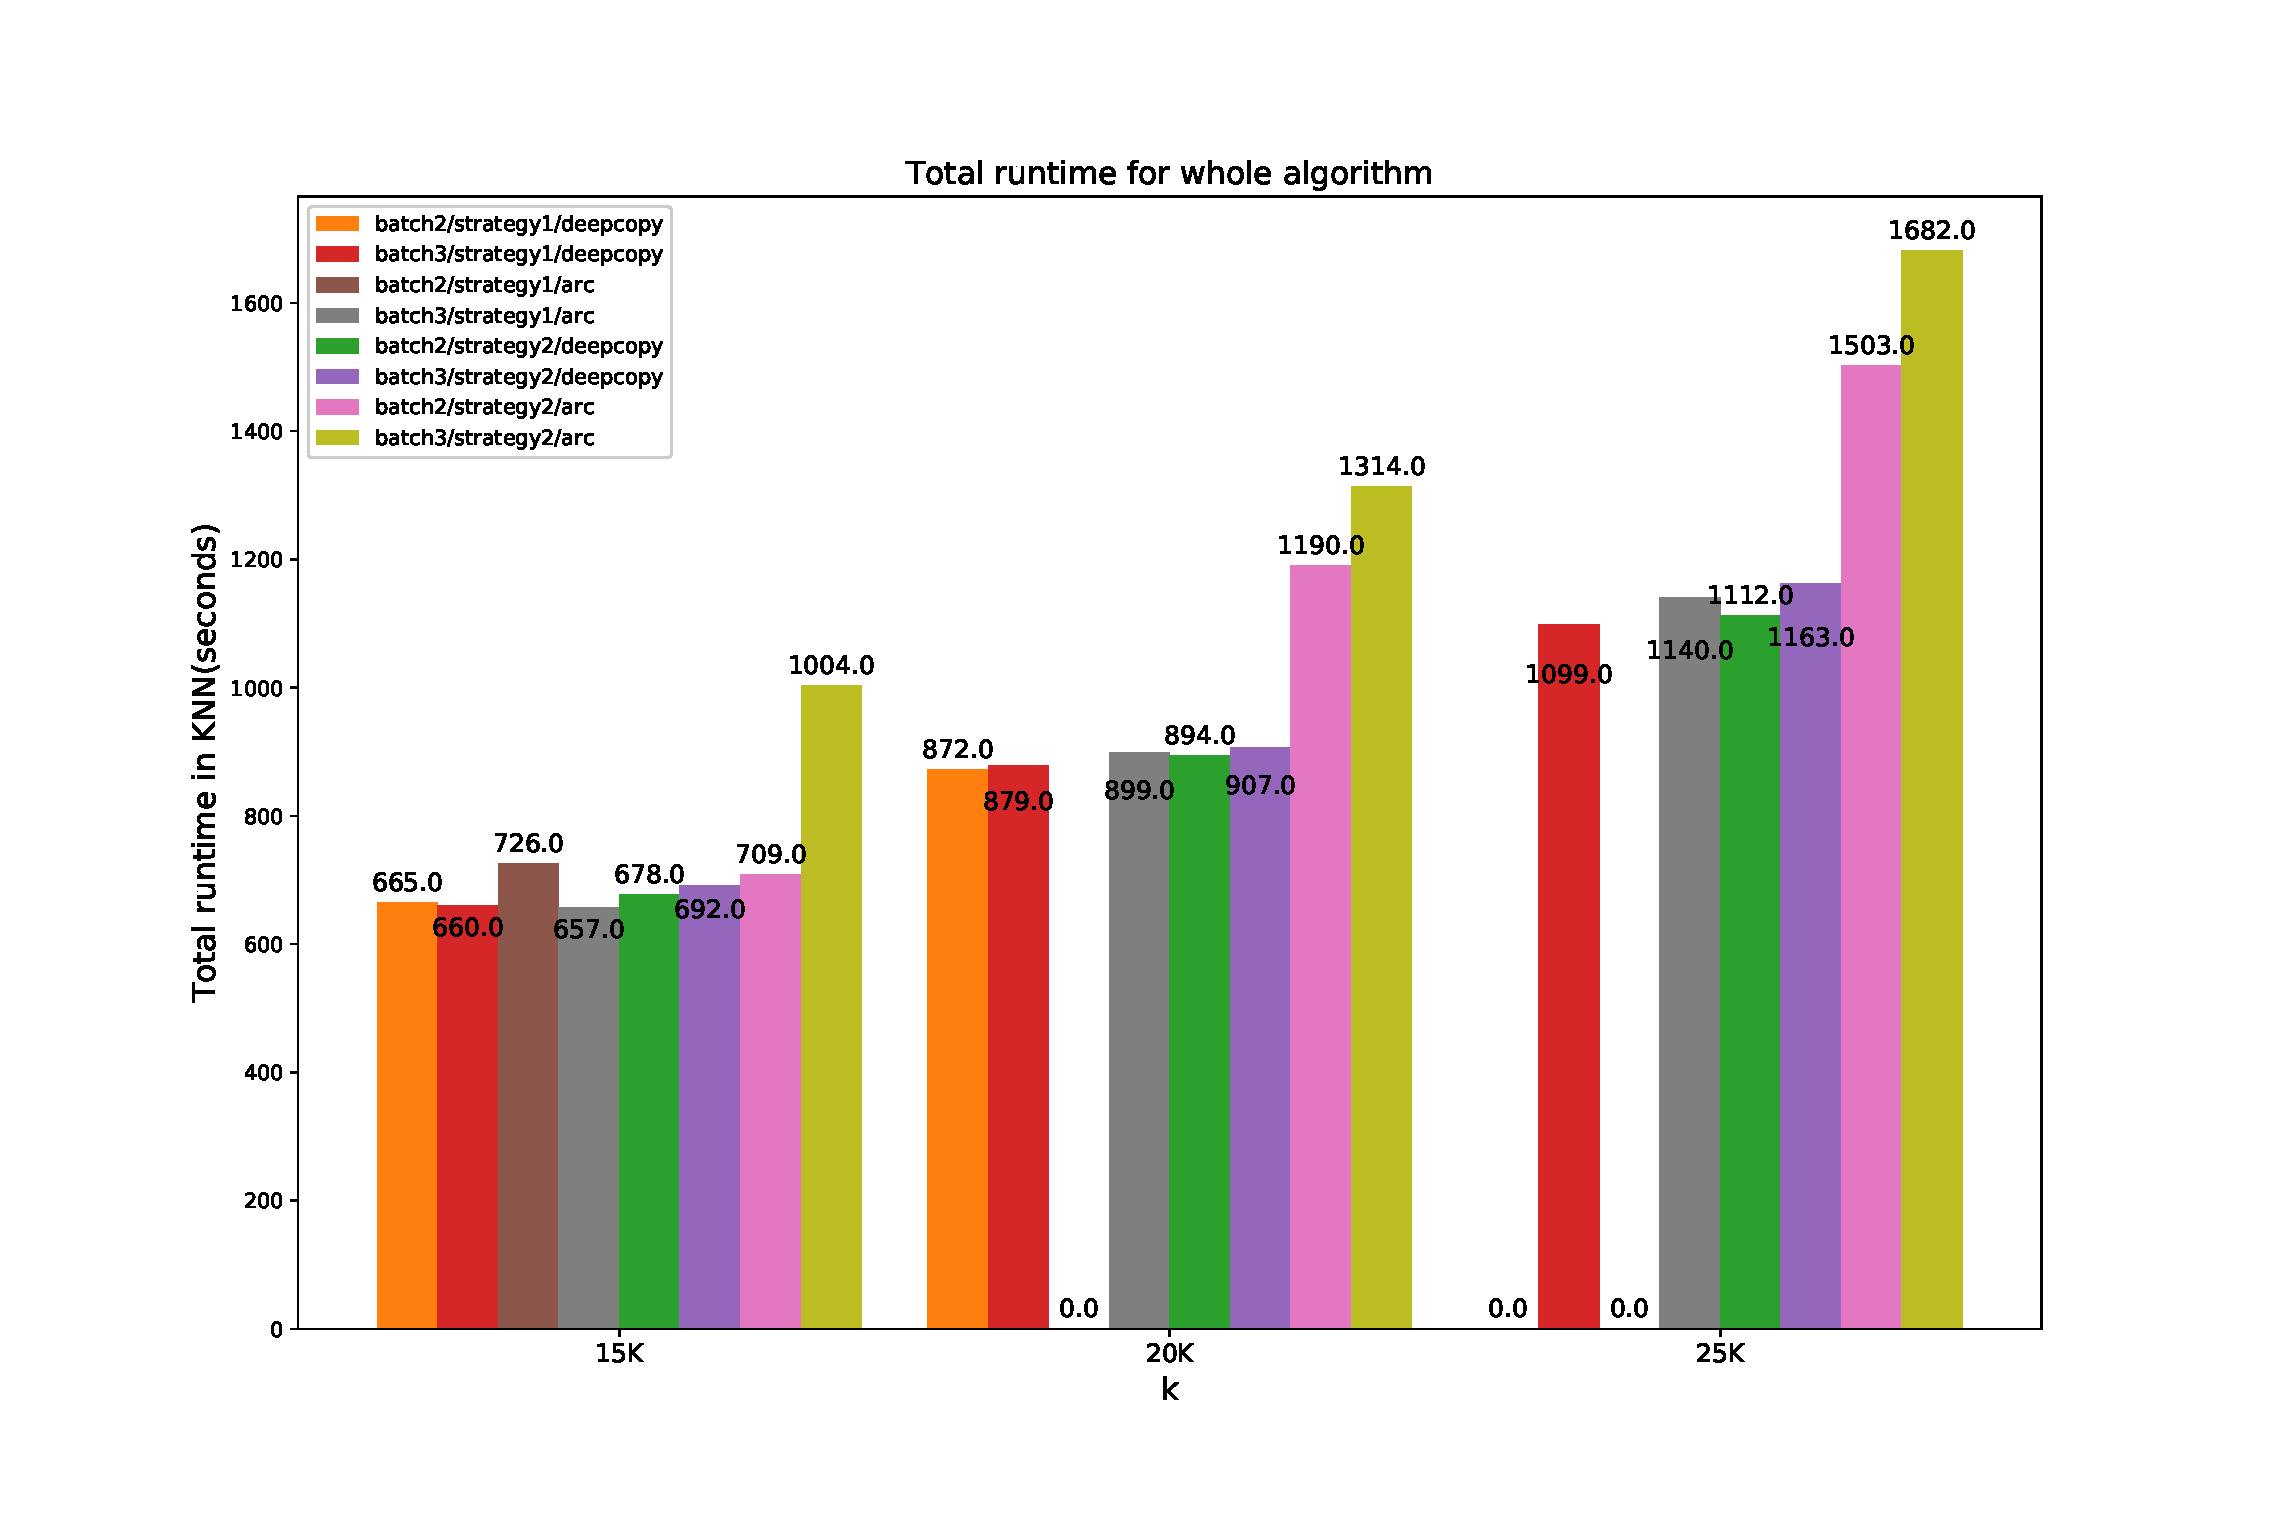
\includegraphics[width=15cm]{total.eps}
    \caption{Total runtime whole KNN algorithm (seconds)}
    \label{fig:total}
\end{figure}

\begin{figure}[htb]
    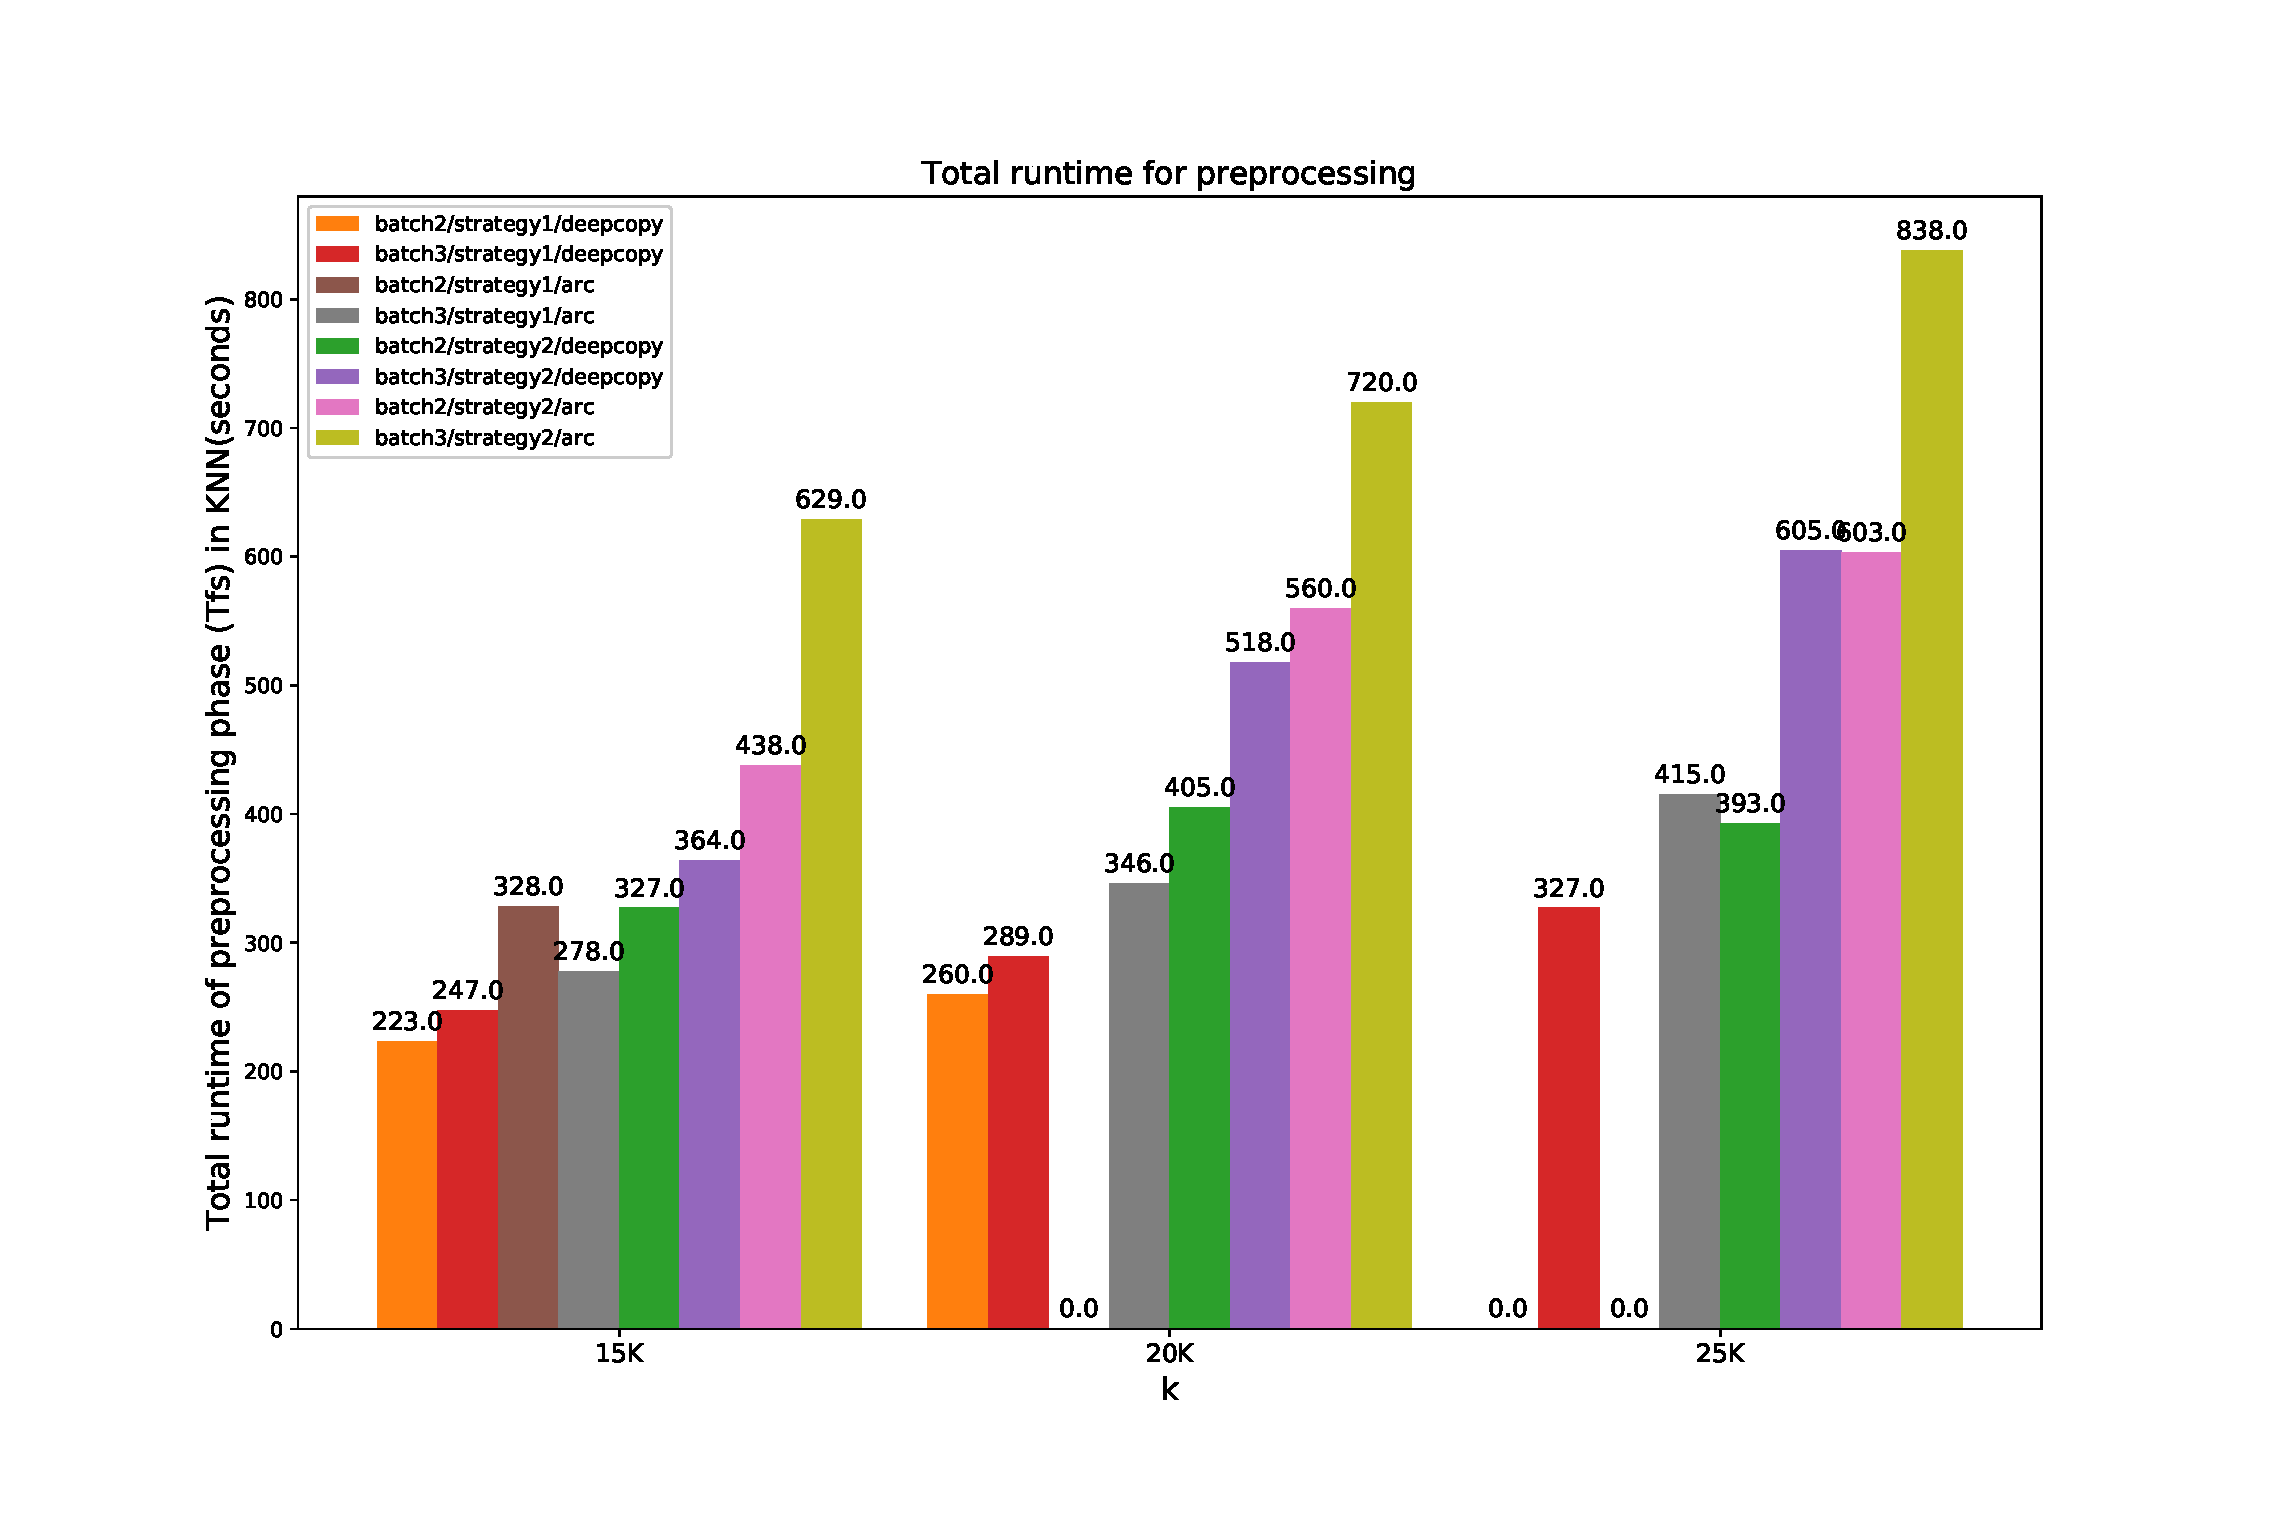
\includegraphics[width=15cm]{preprocessing.eps}
    \caption{Total runtime of preprocessing phase in KNN (seconds)}
    \label{fig:preprocess}
\end{figure}


\begin{figure}[htb]
    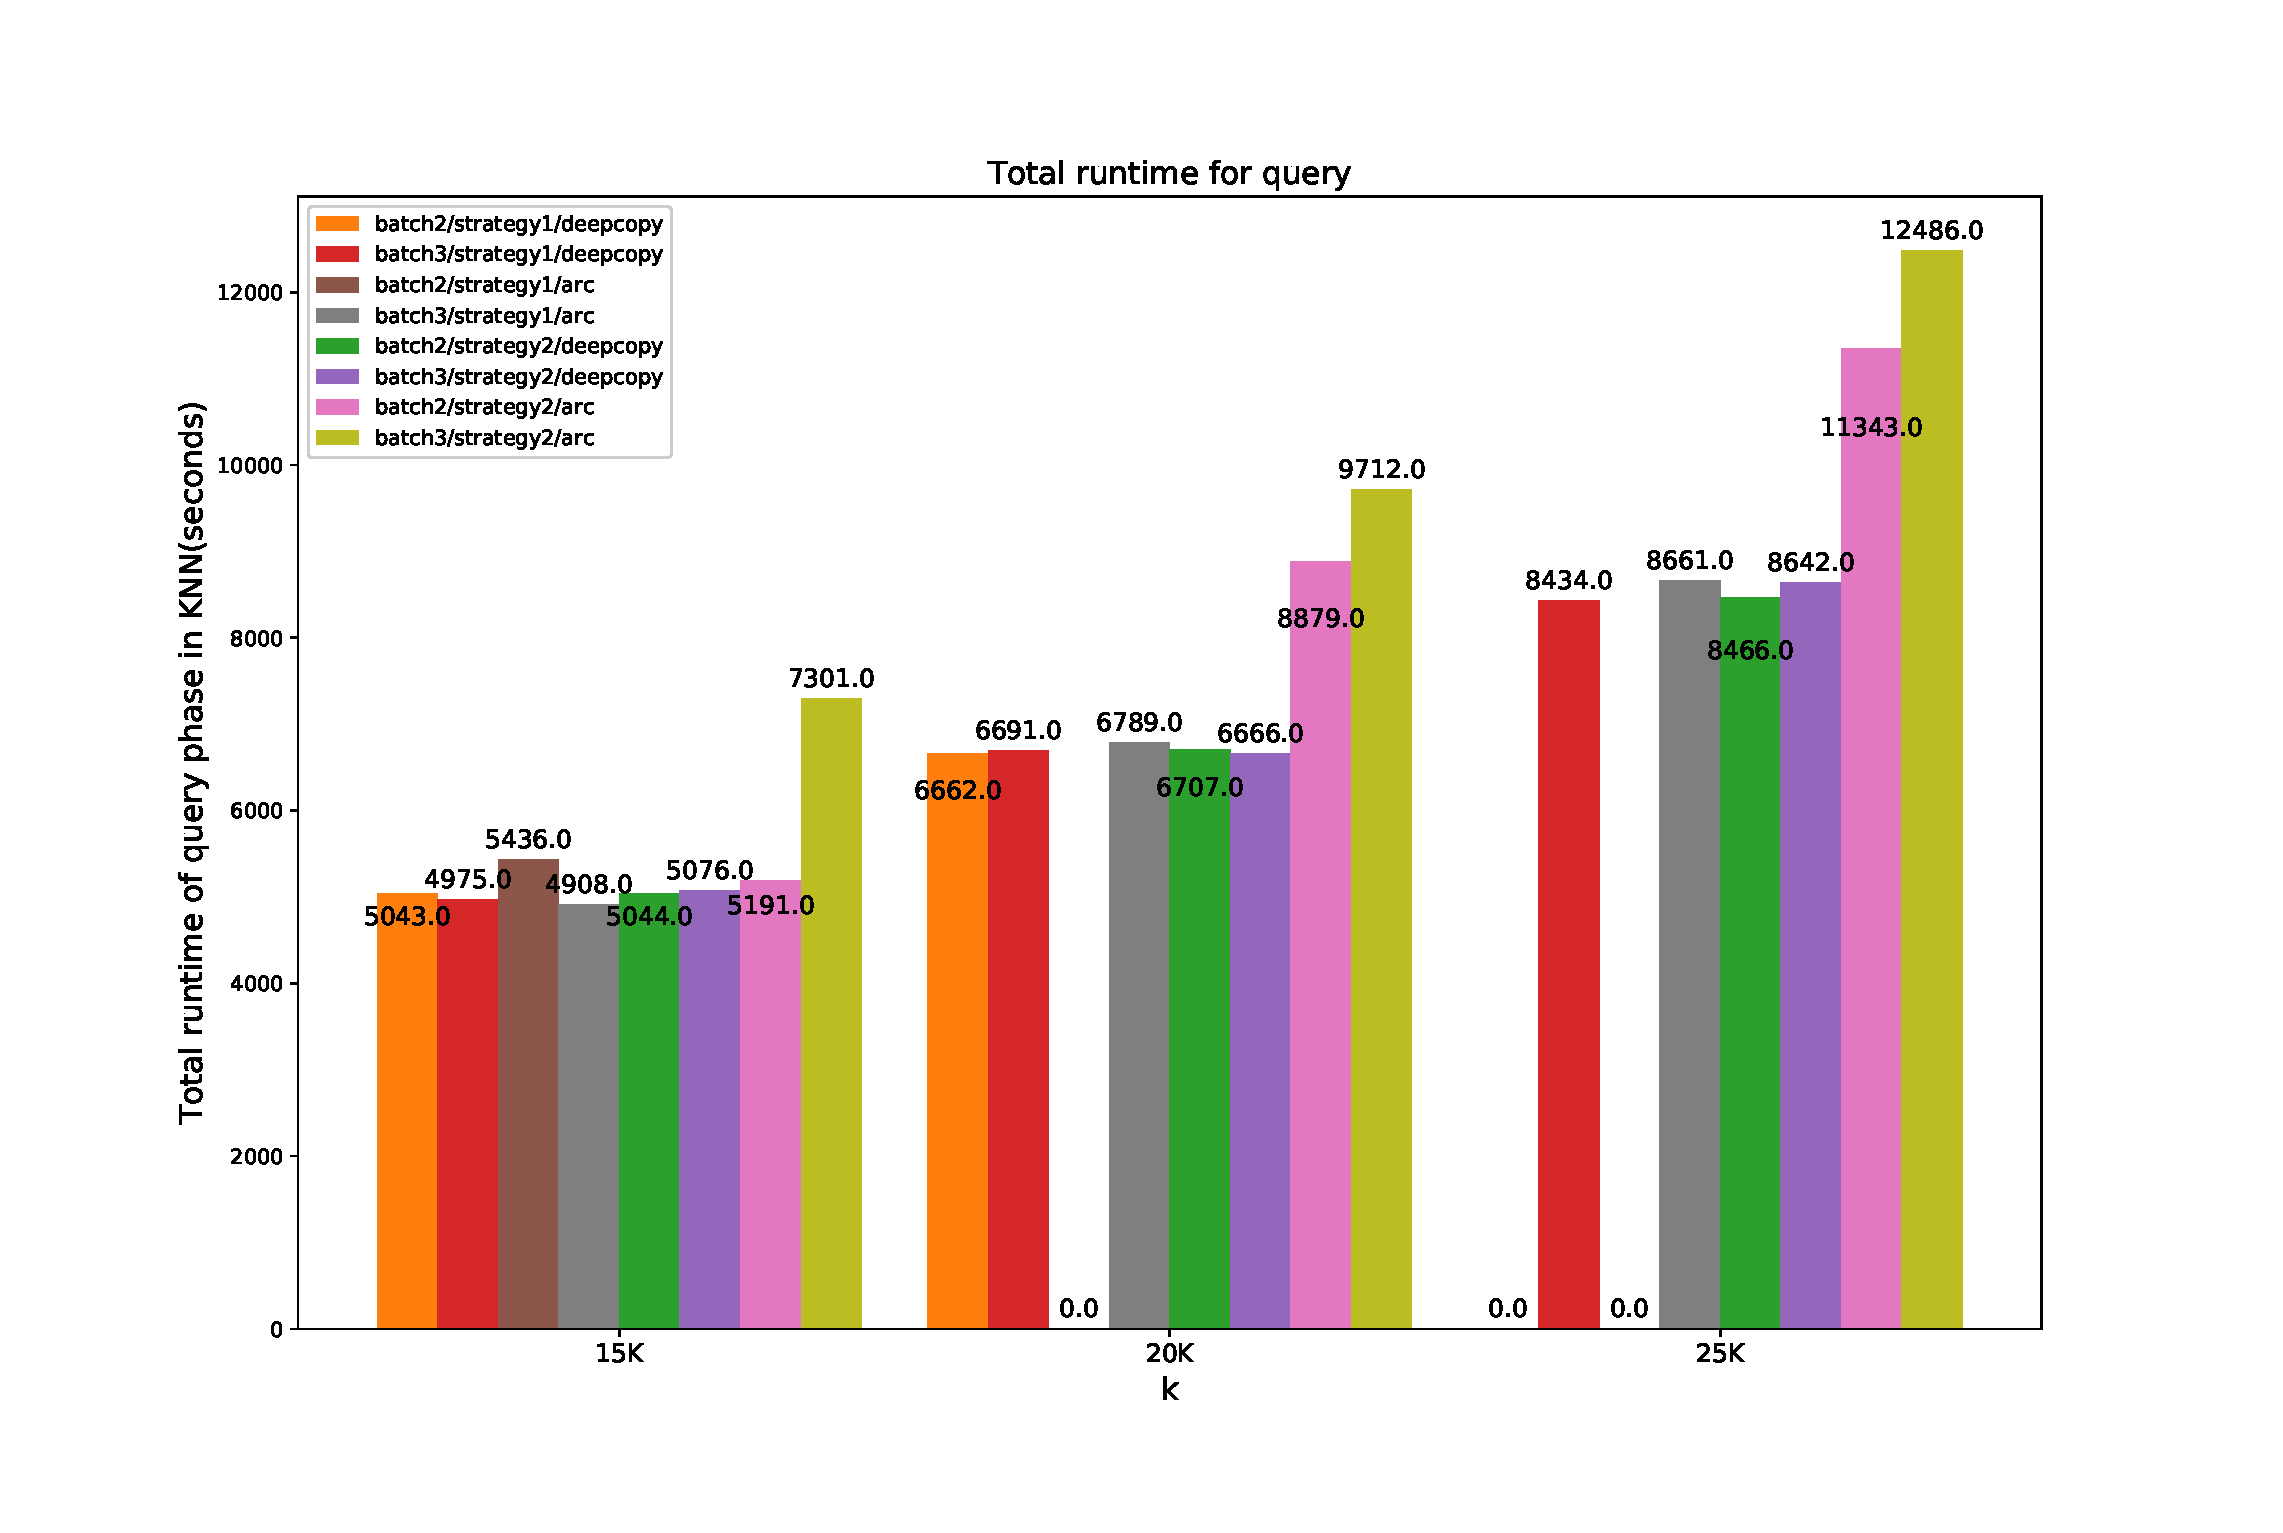
\includegraphics[width=15cm]{query.eps}
    \caption{Total runtime of query phase in KNN (seconds)}
    \label{fig:query}
\end{figure}


